\style{ft}

\section{Mémo \mbpy}

\begin{methode}[Essentiel]
	Importer toutes les fonctions
	~\hfill \pylineGrand{from microbit import *}
	
	Faire une pause {\small(en ms)}
	\hfill \pylineGrand {sleep(...)}\\
\end{methode}



\begin{minipage}[t]{0.6\linewidth}
\begin{methode}[Écrire dans un terminal]
	\rule{-0.25em}{2em}
	Écrire du \textbf{texte} (\texttt{string})
	~\hfill \pylineGrand {print()}\\
	~\hfill \ex \pyline {print('Bouton A : 5 fois')}\\
	
	Aligner avec des \textbf{tabulations}
	~\hfill \pylineGrand {'\t'}\\
	~\hfill \ex \pyline {print('Bouton \tA\t:\t5 fois')}\\
	
	\textbf{Sauter} des lignes
	~\hfill \pylineGrand {'\n'} \\
	~\hfill \ex \pyline {print('Bouton A :\n5 fois\n')}\\
	
	\textbf{Convertir} en chaînes (\texttt{string})
	~\hfill \pylineGrand {str()}\\
	~\hfill \ex \pyline {print('Bouton A :' + str(5) +' fois')}\\
\end{methode}
\end{minipage}
\hfill
\begin{minipage}[t]{0.4\linewidth}
\begin{remarque}
	\rule{-0.25em}{1.7em}
	Activer la \textbf{communication série}\\[0.5em]
	\hfill
	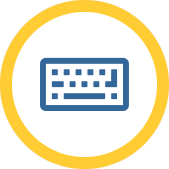
\includegraphics[height=2.5em]{res/ft_repl.png}
	\hfill
	
\includegraphics[height=2.5em]{res/ft_01.png}
	\hfill~
\end{remarque}

\begin{center}
	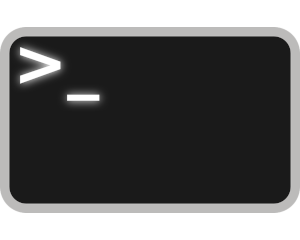
\includegraphics[height=8em]{res/logo-algo.png}
\end{center}
\end{minipage}



\begin{minipage}[t]{0.6\linewidth}
	\begin{methode}[LED \mb]
		\rule{-0.25em}{2em}
		\textbf{Afficher} texte/image
		\hfill \pylineGrand {display.scroll()}\\
		~\hfill \ex \pyline {display.scroll("G")}\\
		~\hfill \ex \pyline {display.scroll(Image.HEART)}\\
		
		Faire \textbf{défiler} texte/image
		\hfill \pylineGrand {display.show()}\\
		~\hfill \ex \pyline {display.show("Gagne !")}\\
		~\hfill \ex \pyline {display.show(Image.HAPPY)}\\
		
		Créer des \textbf{animations}
		\hfill \pylineGrand {delay=...}\\
		~\hfill \ex\pyline {display.show(Image.ALL_CLOCKS, delay=200)}\\
		
		Modifier \textbf{pixel}
		\hfill \pylineGrand {display.set_pixel(x,y,lum)}\\
		\textit{\footnotesize (lum = luminosité $[$0;9$]$)}
		\hfill \ex \pyline {display.set_pixel(0,4,9)}\\
		
		\textbf{Effacer} l'écran
		\hfill \pylineGrand {display.clear()}\\
	\end{methode}
\end{minipage}
\hfill
\begin{minipage}[t]{0.4\linewidth}~\\[1.5em]
\hfill
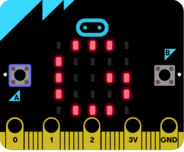
\includegraphics[width=0.35\linewidth]{res/mb-fluctuations-illustration.png}
\hfill
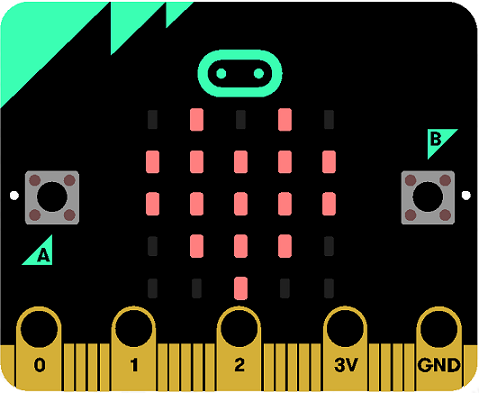
\includegraphics[width=0.35\linewidth]{res/mbpy-init-heart.png}
\hfill~
\\[0em]
\begin{remarque}
	\rule{-0.25em}{1.7em}
	\hfill Pour créer/utiliser des \textbf{animations},\\
	\hfill $\implies$ \textbf{tableaux d'images}.
	
	\ex \pyline{Image.ALL_CLOCKS} (lignes)\\
	\ex \pyline{Image.ALL_ARROWS} (flèches)\\
\end{remarque}	
\end{minipage}

\setlength{\columnsep}{4pt}
\begin{multicols}{4}
	\texttt{Image.HEART}\\
	\texttt{Image.HEART\_SMALL}\\
	\texttt{Image.HAPPY}\\
	\texttt{Image.SMILE}\\
	\texttt{Image.SAD}\\
	\texttt{Image.CONFUSED}\\
	\texttt{Image.ANGRY}\\
	\texttt{Image.ASLEEP}\\
	\texttt{Image.SURPRISED}\\
	\texttt{Image.SILLY}\\
	\texttt{Image.FABULOUS}\\
	\texttt{Image.MEH}\\
	\texttt{Image.YES}\\
	\texttt{Image.NO}\\
	%\columnbreak
	\texttt{Image.CLOCK12}\\
	\texttt{Image.CLOCK11}\\
	\texttt{...}\\
	\texttt{Image.CLOCK1}\\
	\texttt{Image.ARROW\_N}\\
	\texttt{Image.ARROW\_NE}\\
	\texttt{Image.ARROW\_E}\\
	\texttt{Image.ARROW\_SE}\\
	\texttt{Image.ARROW\_S}\\
	\texttt{Image.ARROW\_SW}\\
	\texttt{Image.ARROW\_W}\\
	\texttt{Image.ARROW\_NW}\\
	%\columnbreak
	\texttt{Image.TRIANGLE}\\
	\texttt{Image.TRIANGLE\_LEFT}\\
	\texttt{Image.CHESSBOARD}\\
	\texttt{Image.DIAMOND}\\
	\texttt{Image.DIAMOND\_SMALL}\\
	\texttt{Image.SQUARE}\\
	\texttt{Image.SQUARE\_SMALL}\\
	\texttt{Image.RABBIT}\\
	\texttt{Image.COW}\\
	\texttt{Image.MUSIC\_CROTCHET}\\
	\texttt{Image.MUSIC\_QUAVER}\\
	\texttt{Image.MUSIC\_QUAVERS}\\
	\texttt{Image.PITCHFORK}\\
	\texttt{Image.XMAS}\\
	\texttt{Image.PACMAN}\\
	\texttt{Image.TARGET}\\
	\texttt{Image.TSHIRT}\\
	\texttt{Image.ROLLERSKATE}\\
	\texttt{Image.DUCK}\\
	\texttt{Image.HOUSE}\\
	\texttt{Image.TORTOISE}\\
	\texttt{Image.BUTTERFLY}\\
	\texttt{Image.STICKFIGURE}\\
	\texttt{Image.GHOST}\\
	\texttt{Image.SWORD}\\
	\texttt{Image.GIRAFFE}\\
	\texttt{Image.SKULL}\\
	\texttt{Image.UMBRELLA}\\
	\texttt{Image.SNAKE}
\end{multicols}


\begin{minipage}{0.72\linewidth}
\begin{methode}[Les boutons]
	\rule{-0.25em}{2em}
	Accéder aux \textbf{boutons} A ou B
	\hfill \pylineGrand {button_a. ...}\\
	~\hfill \pylineGrand {button_b. ...}\\

	Nombre d'appuis (\textbf{cumul})
	\hfill \pylineGrand {button_a.get_presses()}\\
	\hfill \pylineGrand {button_b.get_presses()}\\
	\hfill \ex \pyline {display.scroll(str(button_a.get_presses()))}\\
	
	Tester si bouton \textbf{est} pressé
	\hfill \pylineGrand {button_a.is_pressed()}\\
	\hfill \pylineGrand {button_b.is_pressed()}\\
	\hfill \ex \pyline {if (button_b.is_pressed()):print("Bouton B")}\\
	
	Tester si bouton \textbf{a été} pressé
	\hfill \pylineGrand {button_a.was_pressed()}\\
	\textit{\footnotesize (appeler 2 $\times$ la fonction)}
	\hfill \pylineGrand {button_b.was_pressed()}\\
	\hfill \ex \pyline {if (button_b.was_pressed()):display.show(Image.HAPPY)}\\
	
	Utiliser les \textbf{broches}
	\hfill \pylineGrand {pin0.is_touched()}\\
	\hfill \pylineGrand {pin1.is_touched()}\\
	\hfill \pylineGrand {pin2.is_touched()}\\
	
\end{methode}
\end{minipage}
\hfill
\begin{minipage}{0.28\linewidth}
	\begin{center}
		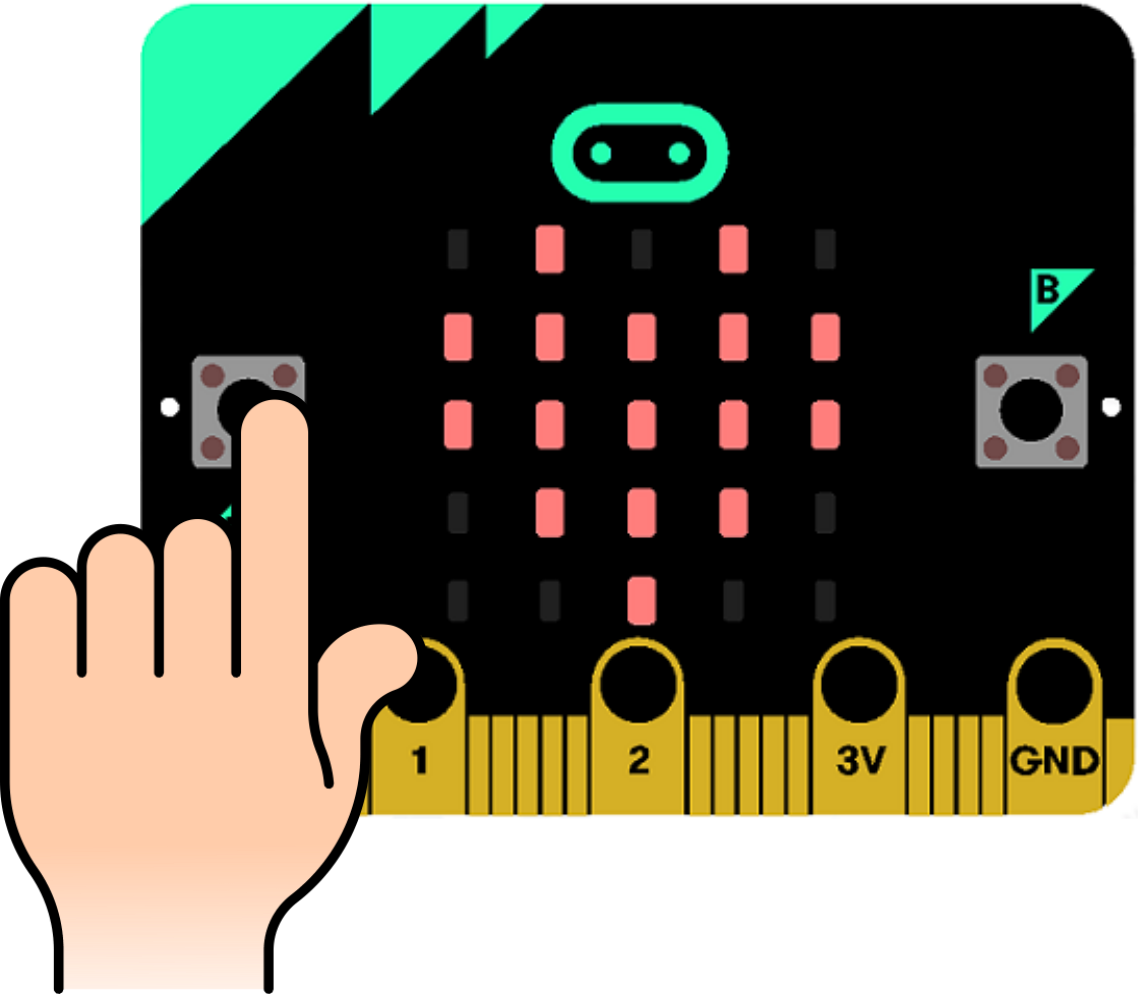
\includegraphics[width=10em]{res/ft_bouton_hand.png}\\[2em]
		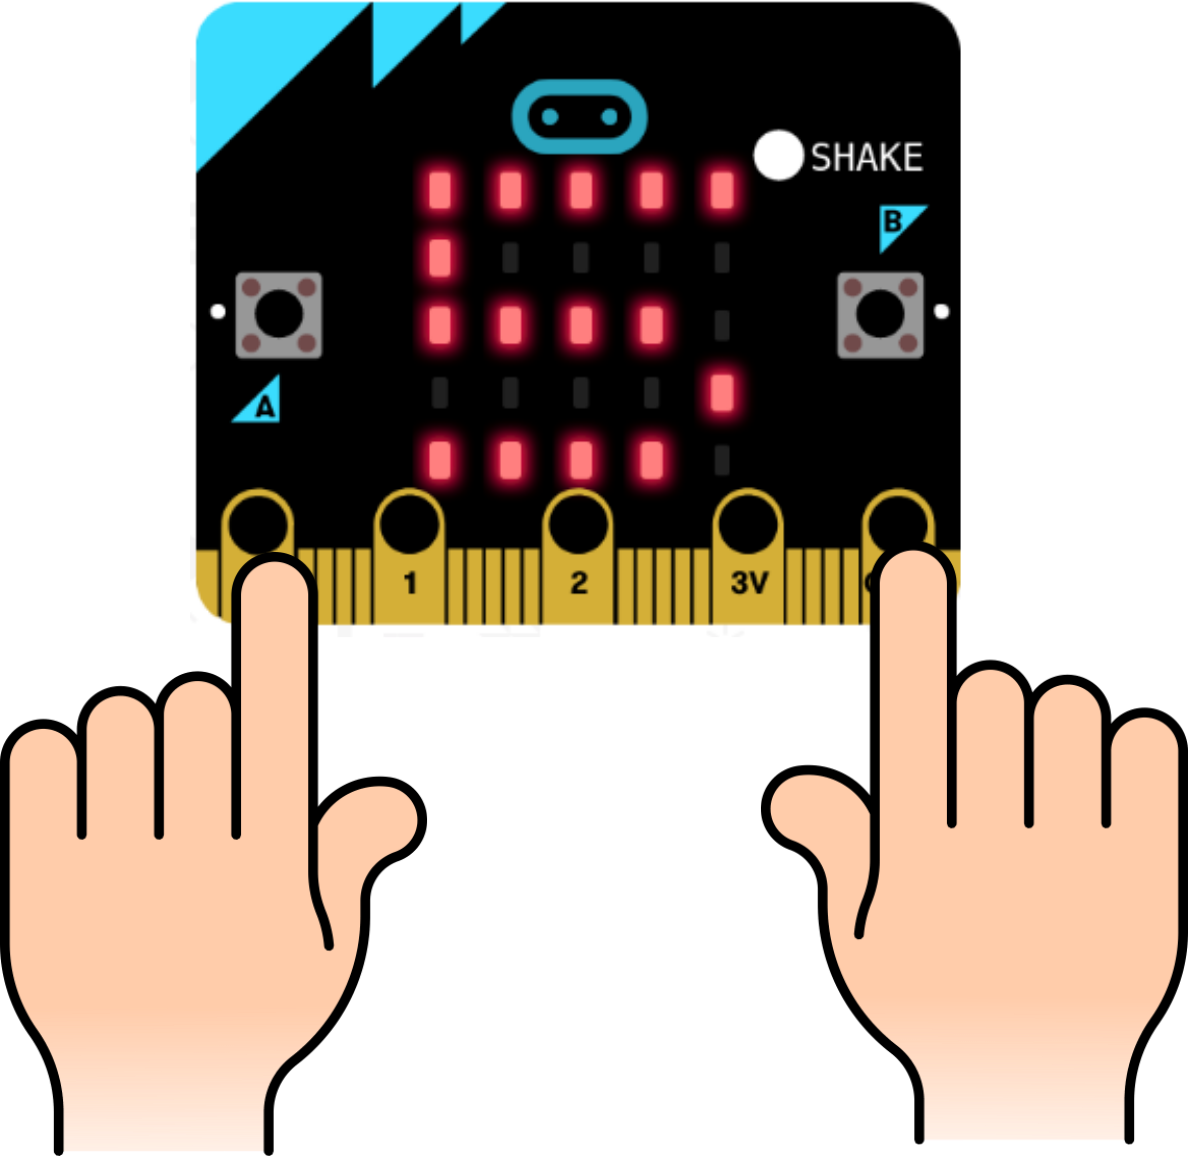
\includegraphics[width=10em]{res/ft_pin_hand.png}
	\end{center}
\end{minipage}

\begin{remarque}
	\rule{-0.25em}{1.7em}
	Détecter un \textbf{évènement}, avec une \textbf{boucle infinie}.
	\hfill	\ex \pyline{while True:}\\
	
	Pour \textbf{sortir d'une boucle} lorsque l'évènement est détecté :
	\hfill \ex \pyline{break}\\
\end{remarque}

\begin{minipage}{0.75\linewidth}
	\begin{methode}[Aléa]
		\rule{-0.25em}{2em}
			Activer le module \textbf{hasard}
			\hfill \pylineGrand{import random}\\
			
			Nombre \textbf{aléatoire} sur $[$0~;~1$]$
			\hfill  \pylineGrand{random.random()}\\
			\hfill \ex \pyline {display.show(round(random.random(),3))}\\
			
			Nombre \textbf{entier} aléatoire sur $[$a ; b$]$
			\hfill  \pylineGrand{random.randint(a,b)}\\
			\hfill \ex \pyline {display.show(random.randint(1,6))}\\
	\end{methode}
\end{minipage}
\hfill 
\begin{minipage}{0.25\linewidth}
	\begin{center}
		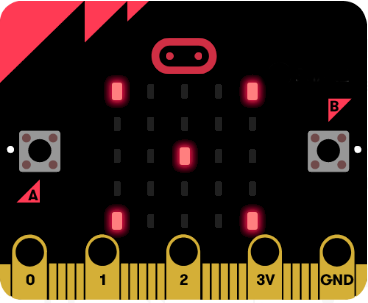
\includegraphics[width=0.8\linewidth]{res/mbpy-de.png}
	\end{center}
\end{minipage}






\begin{minipage}[t]{0.75\linewidth}
	\begin{methode}[Mouvement]
		\rule{-0.25em}{2em}\textbf{1 coord.} vect. accélération
		\hfill \pylineGrand{accelerometer.get_x()}\\
		\hfill \pylineGrand{accelerometer.get_y()}\\
		\hfill \pylineGrand{accelerometer.get_z()}\\
		\hfill \ex \pyline {display.show(accelerometer.get_x())}\\
		
		\textbf{3 coord.} vect. (tuple)
		\hfill \pylineGrand{accelerometer.get_values()}\\
		\hfill \ex \pyline {print(accelerometer.get_values())}\\
		
		Historique \textbf{gestes} (tuple)
		\hfill  \pylineGrand{accelerometer.get_gestures()}\\
		\textit{\footnotesize (appeler 2 $\times$ la fonction)}
		\hfill \ex \pyline {print(accelerometer.get_gestures())}\\
		
		Tester geste \textbf{actuel}
		\hfill  \pylineGrand{accelerometer.is_gesture('...')}\\
		
		Tester geste \textbf{passé}
		\hfill  \pylineGrand{accelerometer.was_gesture('...')}\\
		\textit{\footnotesize (appeler 2 $\times$ la fonction)}		
	\end{methode}
\end{minipage}
\hfill
\begin{minipage}[t]{0.25\linewidth}
	\strut\vspace*{-\baselineskip}\newline
	\begin{center}
		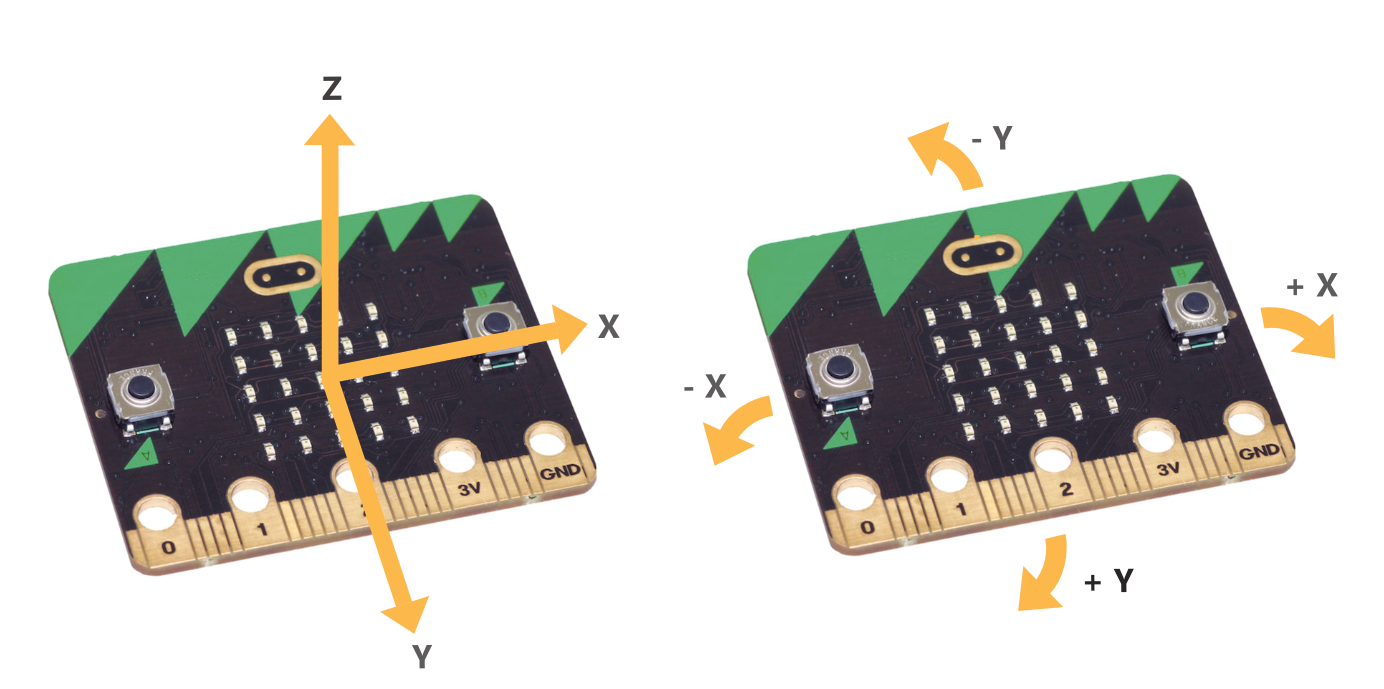
\includegraphics[width=1\linewidth]{res/ft_microbit_axes}
	\end{center}
	
	\textbf{Gestes} reconnus
	\begin{multicols}{2}
		\texttt{'up'}\\
		\texttt{'down'}\\
		\texttt{'left'}\\
		\texttt{'right'}\\
		\texttt{'face up'}\\
		\texttt{'face down'}\\
		\texttt{'freefall'}\\
		\texttt{'3g'}\\
		\texttt{'6g'}\\
		\texttt{'8g'}\\
		\texttt{'shake'}
	\end{multicols}

	\hfill 
\includegraphics[width=0.4\linewidth]{res/mbChutes.png}
\end{minipage}





\begin{minipage}{0.7\linewidth}
	\begin{methode}[Radio]
		\rule{-0.25em}{2em}
		Activer le \textbf{module} radio
		\hfill \pylineGrand{import radio}\\
		
		\textbf{Mettre en route} la radio
		\hfill \pylineGrand{radio.on()}\\
		
		\textbf{Envoyer} un message
		\hfill \pylineGrand{radio.send('...')}\\
		\hfill \ex \pyline{radio.send('pile')}\\
		
		\textbf{Message} reçu (string) 
		\textit{\footnotesize (=\pyline{None}si vide)}
		\hfill \pylineGrand {radio.receive()}\\
		\hfill \ex \pyline {if (radio.receive()=='pile'): print('Pile')}\\
		
		\textbf{Canal} perso $(\leq$ 100$\big )$
		\hfill \pylineGrand{radio.config(channel=..)}\\	
		\hfill \ex \pyline{radio.config(channel=21)}\\
		
		\textbf{Puissance} perso $(\leq$ 7$\big )$
		\hfill \pylineGrand{radio.config(power=..)}\\
		\hfill \ex \pyline{radio.config(power=7)}\\
	\end{methode}
\end{minipage}
\hfill
\begin{minipage}{0.3\linewidth}
	\begin{center}
		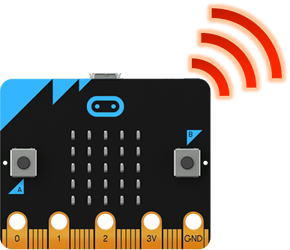
\includegraphics[width=0.7\linewidth]{res/ft_radio.png}\\
	\end{center}
	\hfill \scalebox{-1}[1]{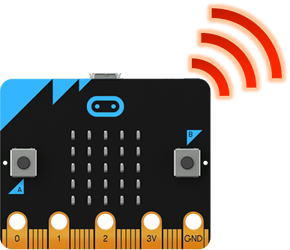
\includegraphics[width=0.2\linewidth]{res/ft_radio.png}}
\end{minipage}




\begin{minipage}{0.6\linewidth}
	\begin{methode}[Boussole]
		\rule{-0.25em}{2em}\textbf{1 coord.} vect. champ magnétique
		\hfill \pylineGrand{compass.get_x()}\\
		\hfill \pylineGrand{compass.get_y()}\\
		\hfill \pylineGrand{compass.get_z()}\\
		\hfill \ex \pyline {display.show(compass.get_x())}\\
		
		\textbf{Angle} (en $^\circ$) avec le nord
		\hfill \pylineGrand{compass.heading()}\\
		\catcode`\%=11
		\hfill \ex \pyline {aiguille=((15-compass.heading())//30)%12}\\
		\catcode`\%=14
		\textbf{Calibrer} la boussole
		\hfill \pylineGrand {compass.calibrate()}\\
	\end{methode}
\end{minipage}
\hfill
\begin{minipage}{0.4\linewidth}
	\begin{center}
		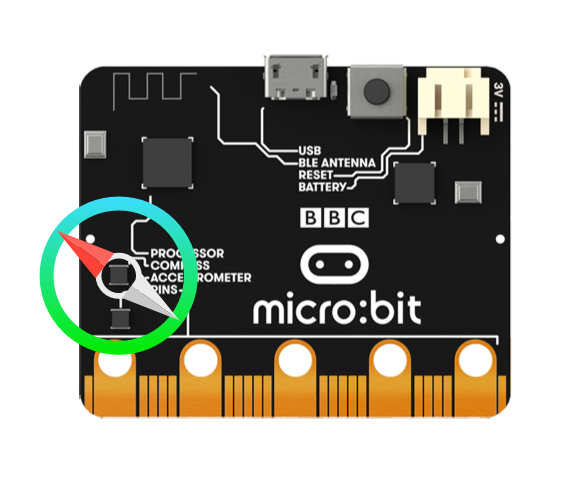
\includegraphics[width=0.4\linewidth]{res/ft_microbit-features-compass.png}
	\end{center}
\begin{remarque}
	\rule{-0.25em}{1.7em}
	\textbf{Toujours} calibrer la boussole.\\[1em]
	
	Mesures/valeurs \textbf{fluctuantes}\\
	{\small(présence de métal, d'aimants, etc.)}
\end{remarque}
\end{minipage}
